\documentclass[a4paper,12pt]{article}

% --- Fundamental Packages ---
\usepackage[utf8]{inputenc}      % Character encoding
\usepackage[T1]{fontenc}         % Font encoding
\usepackage[english]{babel}      % English language (hyphenation, captions, etc.)
\usepackage{geometry}            % Margin management
\geometry{a4paper, top=2.5cm, bottom=2.5cm, left=2.5cm, right=2.5cm}

% --- Math and Images ---
\usepackage{amsmath, amssymb}    % Advanced math formulas
\usepackage{graphicx}            % Image insertion
\usepackage{float}               % Image positioning [H]

% --- Code and Colors ---
\usepackage{listings}            % Source code insertion
\usepackage{xcolor}              % Code coloring

% --- Links and References ---
\usepackage{hyperref}            % Clickable links in PDF
\hypersetup{
    colorlinks=true,
    linkcolor=black,
    filecolor=magenta,      
    urlcolor=blue,
    pdftitle={16 Trucks Report},
    pdfpagemode=FullScreen,
}
\setlength{\parindent}{0pt}

% --- Code Style Definition (Colors) ---
\definecolor{codegreen}{rgb}{0,0.6,0}
\definecolor{codegray}{rgb}{0.5,0.5,0.5}
\definecolor{codepurple}{rgb}{0.58,0,0.82}
\definecolor{backcolour}{rgb}{0.95,0.95,0.92}

% --- MiniZinc Language Definition ---
\lstdefinelanguage{Zinc}{
  keywords={int, float, bool, string, array, set, of, var, par, constraint, solve, satisfy, minimize, maximize, output, include, forall, exists, if, then, else, endif, where, function, predicate},
  sensitive=true,
  morecomment=[l]{\%},
  morestring=[b]",
}

\lstdefinestyle{mystyle}{
    backgroundcolor=\color{backcolour},   
    commentstyle=\color{codegreen},
    keywordstyle=\color{blue}\bfseries,
    numberstyle=\tiny\color{codegray},
    stringstyle=\color{codepurple},
    basicstyle=\ttfamily\small,      % Slightly smaller monospaced font
    breakatwhitespace=false,         
    breaklines=true,                 % Automatic line breaking
    captionpos=b,                    
    keepspaces=true,                 
    numbers=left,                    % Line numbers on the left
    numbersep=5pt,                  
    showspaces=false,                
    showstringspaces=false,
    showtabs=false,                  
    tabsize=2
}

\lstset{style=mystyle, language=Zinc} % Set MiniZinc as default

% --- BEGIN DOCUMENT ---
\begin{document}

% --- TITLE PAGE ---
\begin{titlepage}
    \centering

    % University Header
    {\scshape\LARGE University of Parma \par}
    \vspace{0.5cm}
    {\scshape\Large Department of Mathematical, Physical \par}
    {\scshape\Large and Computer Sciences \par}
    \vspace{0.5cm}
    {\large Master's Degree in Computer Science \par}
    \vspace{1.5cm}

    % Course Name
    {\scshape\Large Constraint Programming course \par}
    \vspace{2cm}

    % Project Title
    {\huge\bfseries Project: 16 - Trucks problem \par}
    \vspace{0.5cm}
    {\Large Modeling, resolution, and benchmark \par}
    \vspace{2cm}

    % Authors
    \large
    \emph{Working group:}\\
    \vspace{0.5cm}

    % Authors Table
    \begin{tabular}{l l}
        \textbf{Samuel Seligardi} & (Student ID: 386xxx) \\
        \textbf{Luca Marchesi}    & (Student ID: 392xxx) \\
        \textbf{Francesco Minei}  & (Student ID: 393xxx) \\
    \end{tabular}

    \vfill

    % Academic Year
    {\large Academic Year 2025/2026 \par}

\end{titlepage}

% --- Table of Contents ---
\tableofcontents
\newpage

\section{Base problem}
The problem is defined on an undirected graph $G=(V,E)$, where $h$ identical objects are distributed over a set of source nodes $S \subseteq V$. A truck, initially located at node $u \in V$, aims to transport all objects to a set of destination nodes $T \subseteq V$. The system is subject to capacity and movement constraints:
\begin{itemize}
    \item The truck can carry at most two objects simultaneously.
    \item If the truck is fully loaded (already carrying two objects), it cannot traverse nodes that contain other objects.
\end{itemize}

The allowed actions at each step are loading an object, unloading one, or moving between adjacent nodes ($cross$). The goal of the base problem is to determine whether a valid plan of length exactly $k$ exists that leads the system from the initial state to a final state where all target nodes $T$ contain at least one object.
\subsection{Model}
The problem is modeled as a CSP (Constraint Satisfaction Problem) over a discrete time horizon. The core of the model relies on a state-space representation that evolves through discrete timesteps, where each step consists of a sequence of logistical actions.

\subsubsection{State representation}
The entire state of the system at any given moment is represented by a decision variable $World$ matrix. This matrix has dimensions $(N+1) \times (k+1)$, where $N$ is the number of nodes in the graph and $k$ is the plan length. The structure of the matrix is defined as follows:
\begin{itemize}
    \item \textbf{Row 0 (The truck):} the first row ($i=0$) represents the truck itself. The value $World[0, t]$ indicates the number of objects currently carried by the truck at timestep $t$ (at the end of the $t$-th transition).
    \item \textbf{Rows 1 to N (The nodes):} each subsequent row $i$ corresponds to a physical node in the graph. The value $World[i, t]$ represents the number of objects located at node $i$ at timestep $t$.
    \item \textbf{Columns (Time):} each column $t$ represents a snapshot of the system state after the $t$-th transition.
\end{itemize}

This representation allows us to enforce the conservation of mass naturally: the sum of all elements in a column $t$ must always equal the total number of objects $h$. While the $World$ matrix tracks the quantities, a sequence of decision variables $S_{pos}[t]$ represents the truck's position. In detail:
\begin{itemize}
    \item \textbf{Definition:} let $S_{pos}[t] \in V$ denote the node index where the truck is located at time $t$.
    \item \textbf{Initial state:} at $t=0$, the position is fixed to the starting node $u$ ($S_{pos}[0] = u$).
    \item \textbf{Trajectory consistency:} the sequence $S_{pos}[0], \dots, S_{pos}[k]$ represents a valid path on the graph, meaning that consecutive positions must be consistent with the graph's topology and the movement actions performed (as defined in the model).
\end{itemize}

\subsubsection{Transition logic: the composite timestep}
Instead of modeling atomic actions (like "move", "load", "unload") as separate timesteps which would unnecessarily increase the horizon $State$ we model a composite timestep. Let $State_t$ denote the system configuration at the end of timestep $t$, defined as the tuple $(S_{pos}[t], World[\cdot, t])$. Each transition from $t-1$ to $t$ consists of a strictly ordered sequence of four logical phases:

$$State_{t-1} \xrightarrow{} Cross_{\epsilon}^* \xrightarrow{} L^* \xrightarrow{} Cross_{\kappa} \xrightarrow{} U^* \xrightarrow{} State_{t}$$

\begin{enumerate}
    \item \textbf{Phase 1: Cross empty ($Cross_{\epsilon}$)}
          If the truck is empty at the beginning of the state ($World[0, t-1]=0$), it is allowed to perform an arbitrary sequence of edge crossing towards a node containing objects. Since we have a connected undirected graph this move can be seen as a teleportation. Specifically, the exact path taken is irrelevant to the model. If the truck is already carrying objects, this phase is skipped, and loading must occur at the current location.

    \item \textbf{Phase 2: Load ($L^*$)}
          The truck can load one or more objects from the current node. The state variables are updated intermediately: objects are subtracted from the node and added to the truck.

    \item \textbf{Phase 3: Cross loaded ($Cross_{K}$)}
          This is the mandatory movement that consumes the physical timestep. The truck, now carrying a payload, moves across an edge of the graph from the loading node to a destination node. This movement must strictly respect the graph's adjacency matrix.

    \item \textbf{Phase 4: Unload ($U^*$)}
          Upon arriving at the destination, the truck may unload one or more objects. The final state at $t$ reflects the distribution of objects after this unloading phase.
\end{enumerate}

\subsection{Implementation}

\subsubsection{Key constraints}
The model is built upon a set of fundamental constraints that enforce the physical and logical rules of the problem:

\paragraph{Conservation constraint} The total number of objects in the system remains constant throughout all timesteps. This is expressed as:
$$\sum_{i=0}^{N} World[i, t] = h \quad \forall t \in [0, k]$$
where $h$ is the total number of objects. This constraint ensures that objects are neither created nor destroyed during the plan execution.

\paragraph{Capacity constraint} The truck has a hard capacity limit of 2 objects, enforced at all timesteps:
$$World[0, t] \le 2 \quad \forall t \in [0, k]$$
This constraint directly limits the first row of the state matrix, preventing the truck from carrying more than two objects simultaneously.

\paragraph{Adjacency constraint} The mandatory movement phase (Cross$_K$) must respect the graph topology. For each timestep $t$, if the truck moves from node $load\_node[t]$ to node $S_{pos}[t]$, then:
$$Adj[load\_node[t], S_{pos}[t]] = 1$$
where $Adj$ is the adjacency matrix of the undirected graph. This ensures that the truck only traverses edges that exist in the graph.

\paragraph{Cross$_\epsilon$ teleportation} When the truck is empty at the beginning of a timestep ($World[0, t-1] = 0$), it can move to any node containing objects without consuming the timestep. This is modeled as a "teleportation" action: the truck appears at a loading node $load\_node[t]$ where objects are available for pickup. The specific path taken is irrelevant, as only the final position matters.

\paragraph{Full truck blocking rule} A critical constraint enforces that a fully loaded truck cannot simply pass through occupied nodes. Formally, if the truck arrives at destination node $S_{pos}[t]$ carrying 2 objects, and $World[S_{pos}[t], t-1] > 0$ (the node was occupied before unloading), then:
$$unloaded[t] \ge 1$$
This forces the truck to unload at least one object before it can leave, preventing traversal of occupied nodes while maintaining full capacity. Furthermore, at the following timestep, the truck cannot load again until it has moved to a different node.

\paragraph{Goal constraint} At the final timestep $k$, all target nodes in $T$ must contain at least one object:
$$World[i, k] \ge 1 \quad \forall i \in T$$
This ensures that the plan successfully achieves the objective of delivering objects to all designated destinations.

\subsubsection{Implementation choices}

\paragraph{From plan\_length to incremental $k$ approach}
The initial model design included a decision variable $plan\_length$ representing the actual length of the plan, with the objective function:
$$\text{minimize } plan\_length \text{ subject to } plan\_length \le k$$
The goal was to find the shortest valid plan within the maximum horizon $k$. However, the benchmark methodology employs an incremental approach: it tests $k=1, 2, 3, \ldots, k_{max}$ sequentially, stopping at the first value where a solution exists, with a timeout of 300 seconds per instance. A key insight emerged: if a solution exists for some $k=y < x$, the incremental search would already find it during iteration $k=y$. When the solver reaches $k=x > y$, any feasible plan already represents the minimal length plan for that instance. Therefore, the $plan\_length$ variable becomes redundant, minimizing it provides no additional value. The final implementation removes the $plan\_length$ variable entirely and uses a pure satisfiability approach with \texttt{solve satisfy}. This design decision:
\begin{itemize}
    \item Reduces the search space by eliminating an unnecessary optimization variable
    \item Simplifies the model, making it easier for the solver to reason about
    \item Avoids redundant optimization when the incremental framework already identifies minimal plans
    \item Improves runtime by focusing purely on feasibility rather than optimality
\end{itemize}

\paragraph{Solver Selection}
Extensive testing was conducted with four different solvers: Chuffed, Gecode, HiGHs, and OR-Tools. Chuffed demonstrated significantly superior performance on this scheduling problem, consistently achieving lower runtimes and solving all 100 benchmark instances without timeout.

The rationale for Chuffed's effectiveness lies in its \textit{lazy clause generation} mechanism, which combines conflict-driven clause learning from SAT solving with constraint propagation. Scheduling problems like the this one involve complex temporal dependencies and resource constraints that benefit greatly from learned clauses. In contrast, traditional CP solvers like Gecode rely primarily on propagation and search heuristics, which are less effective at identifying and exploiting patterns in the constraint structure. HiGHs and OR-Tools were also evaluated to provide a comprehensive comparison. While OR-Tools achieved a 100\% success rate, its average runtime was approximately twice that of Chuffed, confirming Chuffed as the optimal solver choice for this problem class.

\paragraph{Constraint Optimization}
The final model incorporates several optimizations to leverage Chuffed's strengths:
\begin{itemize}
    \item Heavy use of reification to model conditional constraints (e.g., $had\_cross\_e[t]$, $must\_unload[t]$)
    \item Decomposition of complex transitions into atomic phases with intermediate state variables
    \item Explicit modeling of load/unload quantities to enable better propagation
    \item Channeling constraints between $S_{pos}$ and $World$ matrix to strengthen propagation
\end{itemize}

\subsection{Results}

This section presents the experimental evaluation of the base problem across four solvers and multiple search strategies. All benchmarks were conducted on a suite of 100 instances with varying graph sizes (N = 10, 14, 18, 22, 26) and plan lengths (k = 5, 8, 11, 14, 17). Each instance was subject to a 300-second timeout.

\subsubsection{Solver Comparison}

Table~\ref{tab:base-solver-stats} summarizes the performance of all four solvers on the base problem.

\begin{table}[H]
    \centering
    \caption{Solver performance comparison on base problem (100 instances, 300s timeout)}
    \label{tab:base-solver-stats}
    \begin{tabular}{|l|c|c|c|c|}
        \hline
        \textbf{Solver} & \textbf{Solved} & \textbf{Timeouts} & \textbf{Avg Time (s)} & \textbf{Success \%} \\
        \hline
        Chuffed         & 100/100         & 0                 & 1.85                  & 100.0\%             \\
        Gecode          & 86/100          & 14                & 53.49 (13.36)         & 86.0\%              \\
        HiGHs           & 75/100          & 25                & 93.70 (24.93)         & 75.0\%              \\
        OR-Tools        & 100/100         & 0                 & 3.96                  & 100.0\%             \\
        \hline
    \end{tabular}
\end{table}

Chuffed emerges as the clear winner, solving all instances with an average runtime of just 1.85 seconds. OR-Tools also achieves a perfect success rate but with double the average runtime of Chuffed (3.96s). The high timeout rates for Gecode (14\%) and HiGHs (25\%) indicate that these solvers struggle with the harder instances in the benchmark suite, particularly those involving larger graphs and longer plan horizons.

For Gecode and HiGHs, the values in parentheses represent the average runtime computed only over successfully solved instances, excluding timeouts. This provides a fairer comparison of solver efficiency when the success rates differ significantly. Considering only successful instances, Chuffed (1.85s) is approximately 7 times faster than Gecode (13.36s) and over 13 times faster than HiGHs (24.93s). The non parenthesized values include timeouts counted as 300 seconds, resulting in higher overall averages of 53.49s for Gecode and 93.70s for HiGHs.

Figure~\ref{fig:base-solver-comparison} visualizes the runtime distribution across all instances for each solver, including timeouts (shown as 300-second bars). The plot clearly shows Chuffed's consistently low runtimes and tight distribution, while Gecode and HiGHs exhibit much higher variance, median runtimes, and multiple timeout instances.

\begin{figure}[H]
    \centering
    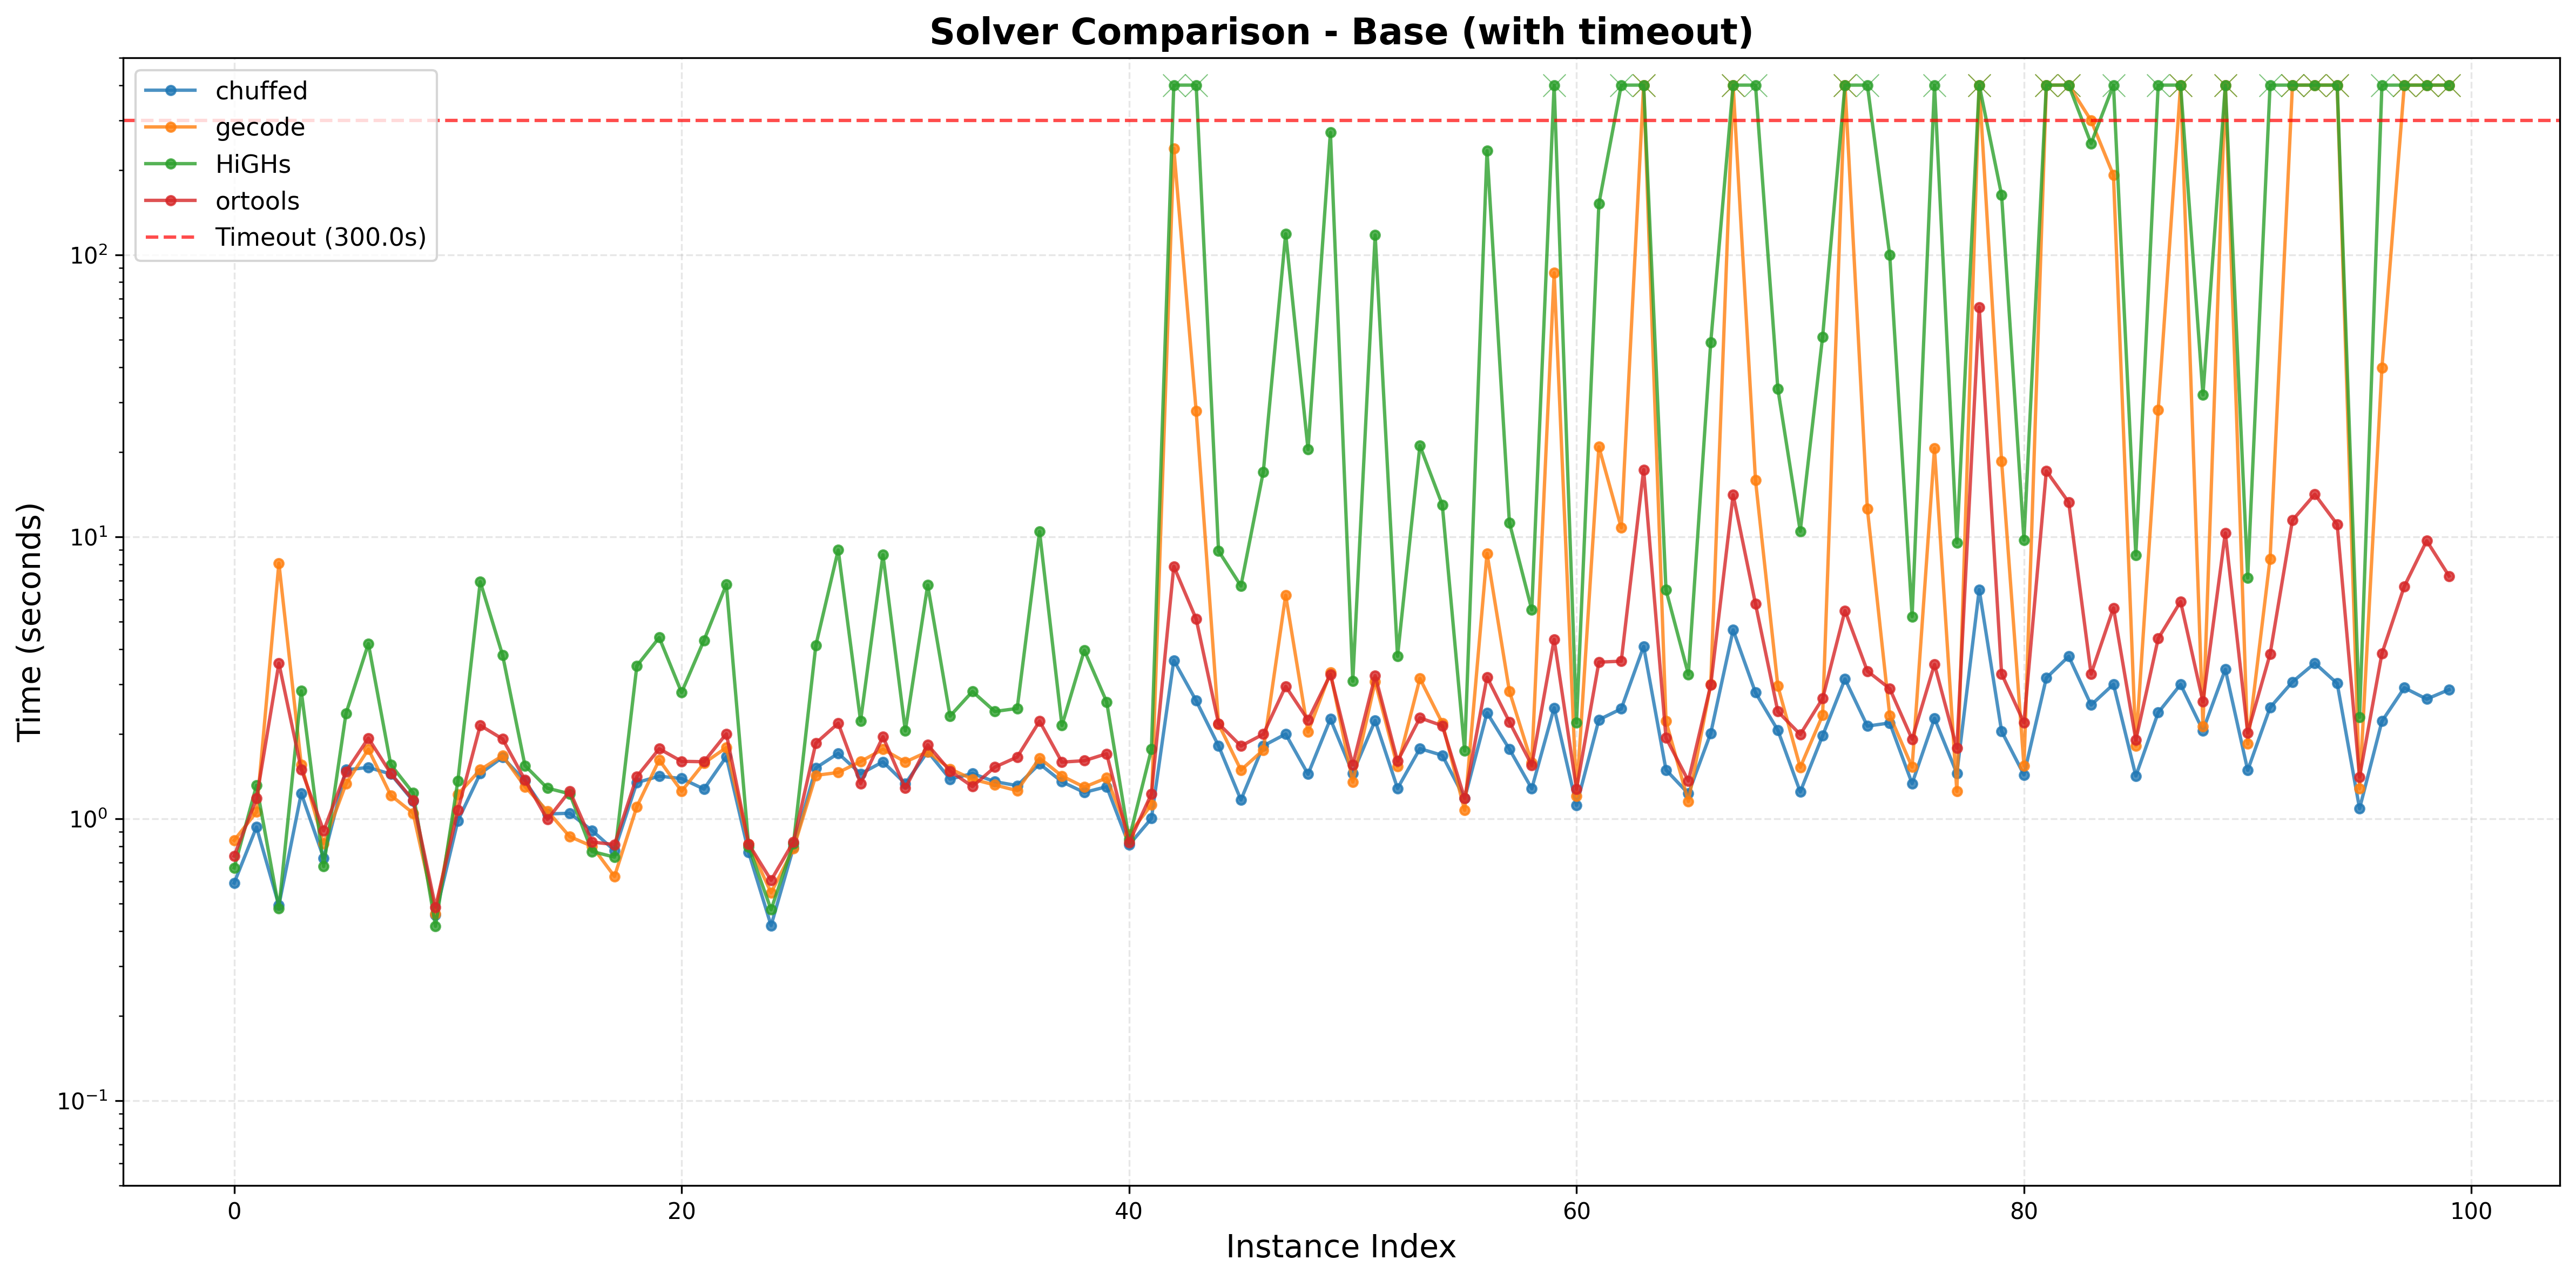
\includegraphics[width=0.85\textwidth]{figures/solver_comparison_base_full.png}
    \caption{Solver comparison on base problem (including timeouts)}
    \label{fig:base-solver-comparison}
\end{figure}

\subsubsection{Search Strategy Analysis}

Beyond solver selection, we evaluated the impact of custom search strategies on Chuffed's performance. Figure~\ref{fig:base-strategies} compares 12 different search annotation strategies against Chuffed's default configuration.

\begin{figure}[H]
    \centering
    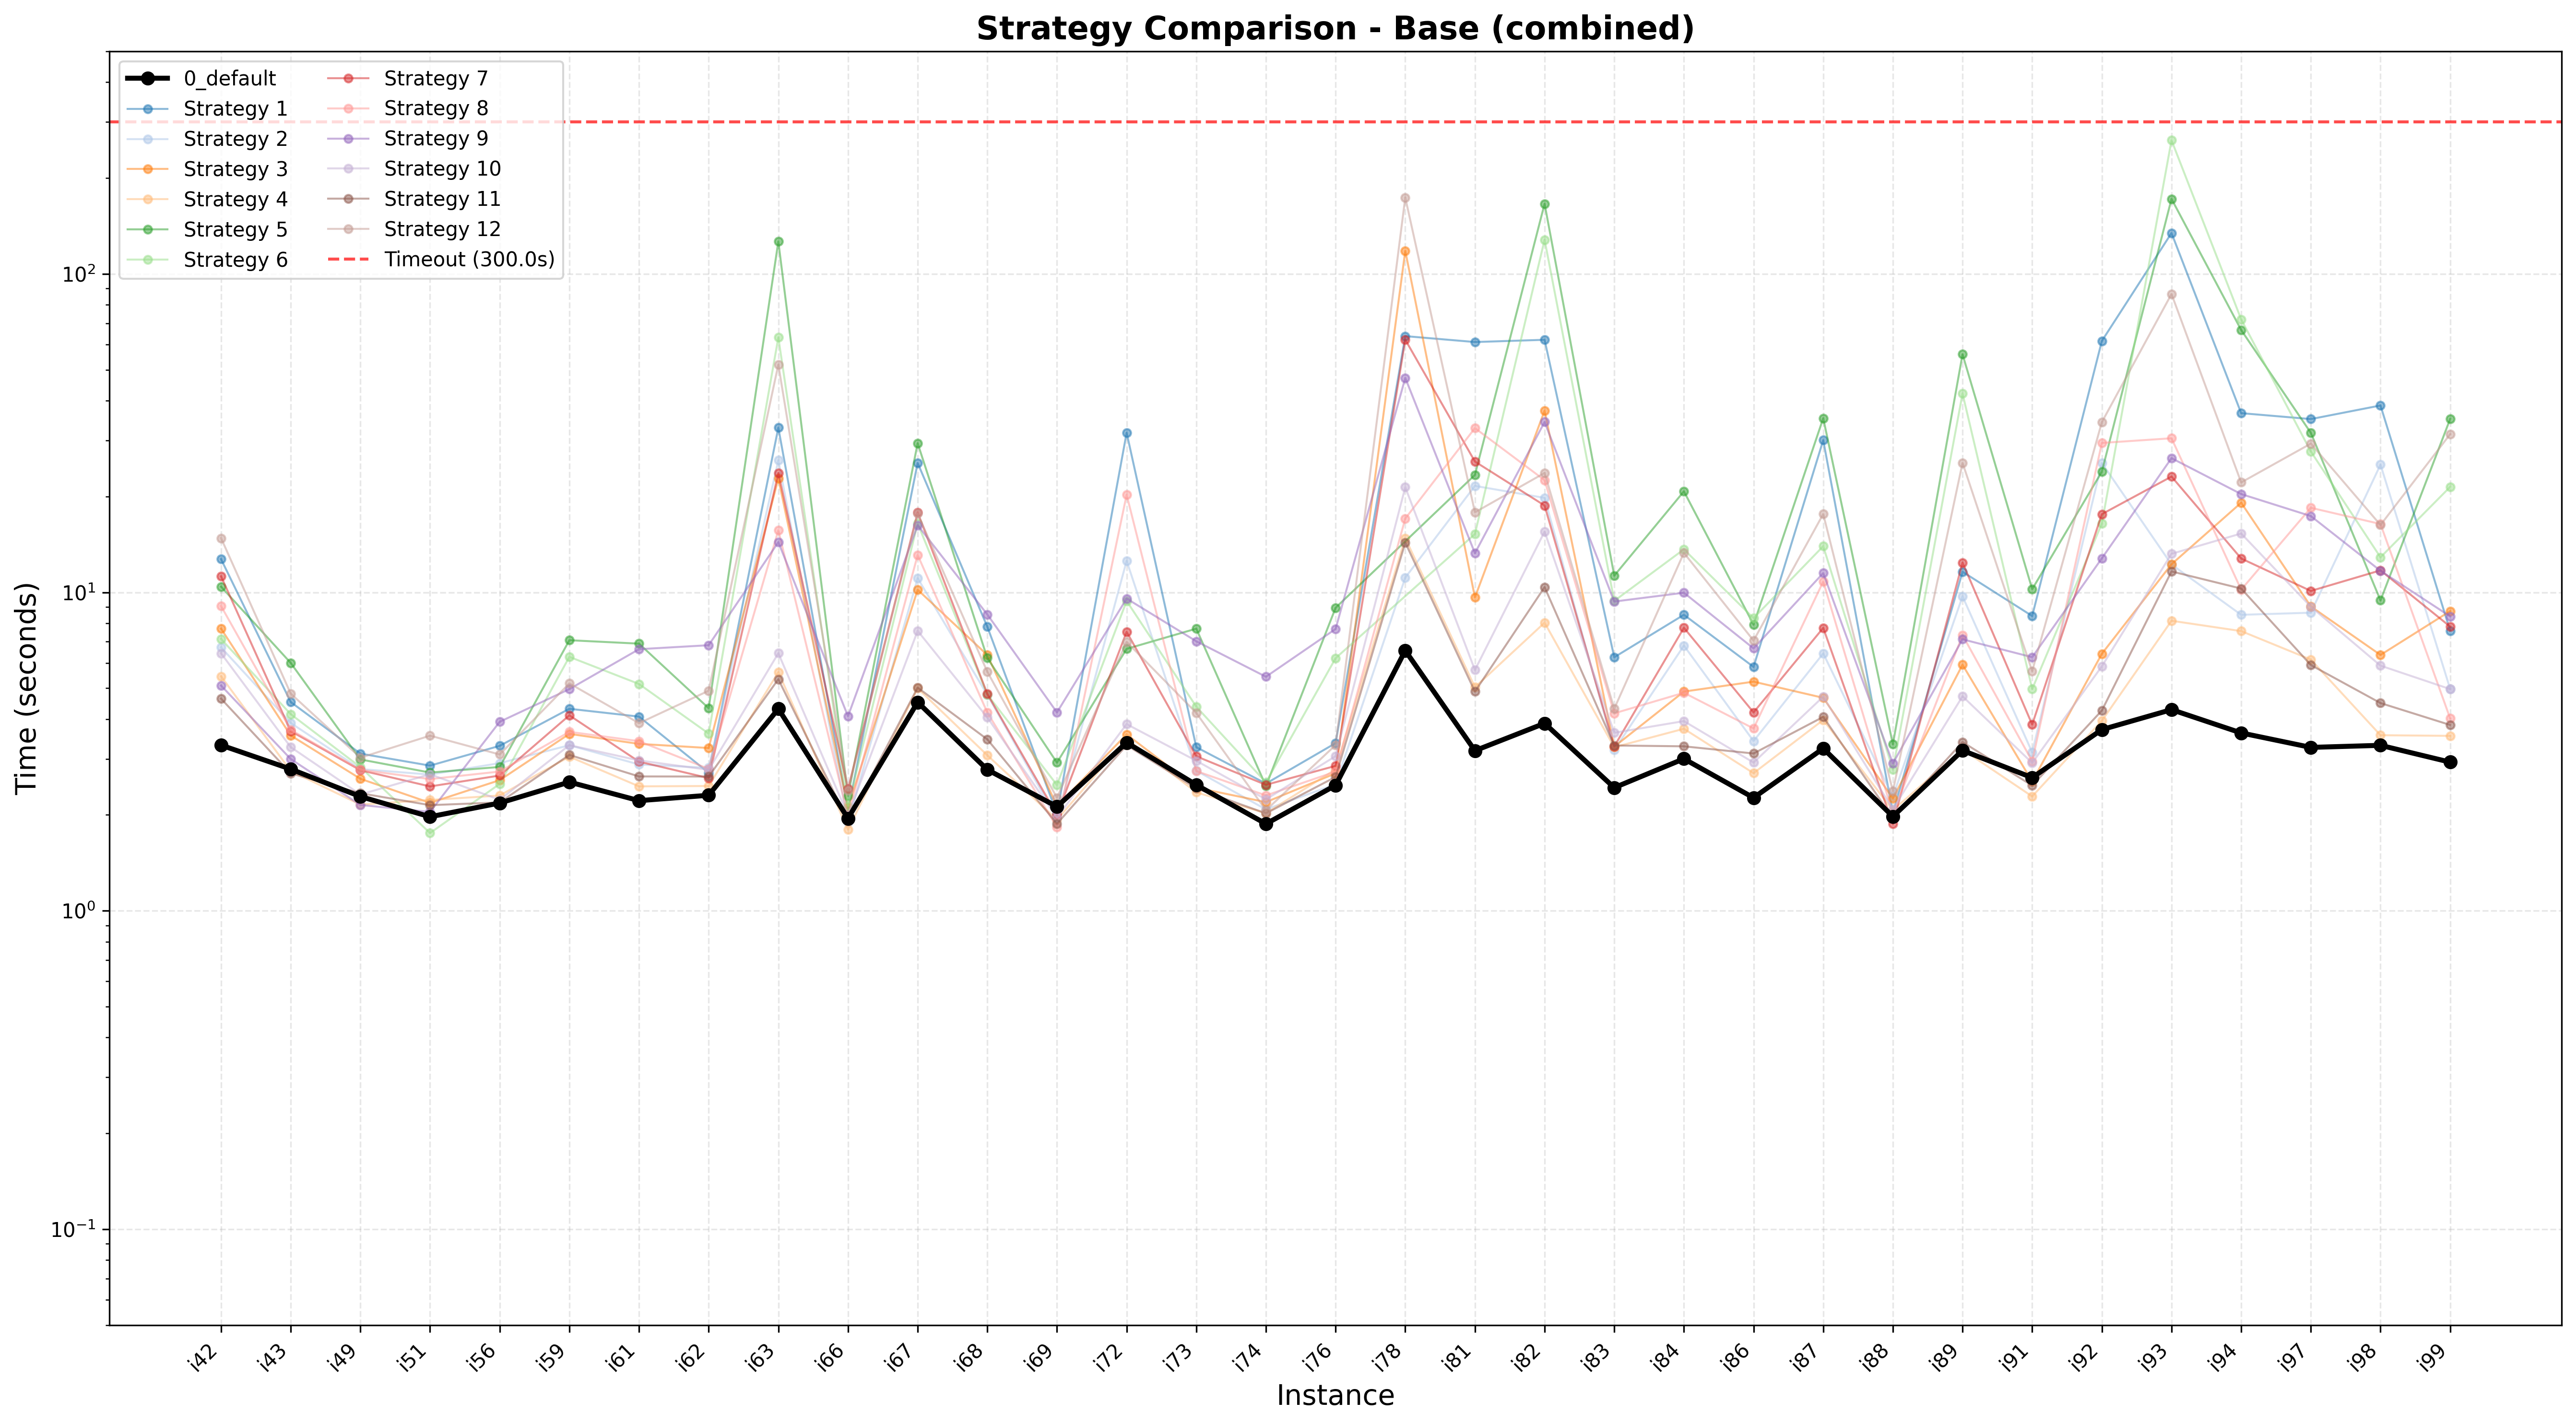
\includegraphics[width=0.85\textwidth]{figures/strategy_combined_base_full.png}
    \caption{Search strategies comparison on base problem (including timeouts)}
    \label{fig:base-strategies}
\end{figure}

The results reveal a somewhat surprising conclusion: Chuffed's default search strategy performs competitively with, and often outperforms, manually designed custom strategies. Strategies such as sequential-timestep ordering, position-first variable selection, and adaptive domain splitting show marginal differences from the default, with no strategy providing a consistent, significant improvement. This finding suggests that Chuffed's internal heuristics and lazy clause generation mechanism are already well-tuned for this problem structure. The solver automatically learns and exploits patterns during search, reducing the need for hand-crafted annotations. For practitioners, this means the default configuration is a robust starting point, eliminating the time-consuming process of strategy tuning.

\subsubsection{Scaling Behavior}

An analysis of runtimes across different graph sizes reveals that performance degrades as the problem scale increases. Instances with N=10 nodes typically solve in under 2 seconds with Chuffed, while instances with N=26 nodes can take up to 10-20 seconds. The timeout instances for Gecode and HiGHs are predominantly concentrated in the larger graph sizes (N $\ge$ 18), confirming that Chuffed's lazy clause generation provides a distinct advantage on harder, more structured instances.

\section{Minimization problem}

The minimization problem extends the base formulation by introducing a cost function over the plan. Given a fixed plan length $k$ (typically the minimum value found by the base problem), the objective is to find a valid plan that minimizes the total travel cost.

\subsection{Model}

The minimization model builds upon the base problem's state representation and transition logic, adding a cost structure to quantify the "expense" of movements.

\subsubsection{Distance Matrix}

A key addition is the distance matrix $Dist[i, j]$ for all $i, j \in \{1, \ldots, N\}$, representing the shortest path length between any pair of nodes. This matrix is precomputed using the Dijkstra algorithm on the graph's adjacency matrix and stored in the instance's \texttt{.dzn} file. The distance metric provides a natural cost function: moving between non-adjacent nodes incurs a cost proportional to the shortest path connecting them.

\subsubsection{Cost Function}

The total cost of a plan is composed of two types of movements:

\paragraph{Cross$_\epsilon$ Cost} When the truck is empty and "teleports" to a loading node, the cost is the shortest path distance:
$$cost\_cross\_e[t] = Dist[S_{pos}[t-1], load\_node[t]]$$

\paragraph{Cross$_K$ Cost} The mandatory loaded movement incurs a weighted cost:
$$cost\_cross\_k[t] = Dist[load\_node[t], S_{pos}[t]] \times cross\_k\_weight$$
where $cross\_k\_weight = 2$. The weight factor reflects the intuition that moving with a payload is more "expensive" than empty movement, it represents the actual physical traversal that consumes the timestep and must respect adjacency constraints.

\paragraph{Total Cost} The objective to minimize is the sum of all movement costs across the plan:
$$total\_cost = \sum_{t=1}^{k} \left( cost\_cross\_e[t] + cost\_cross\_k[t] \right)$$

The optimization problem is formulated as:
$$\text{minimize } total\_cost \text{ subject to all base problem constraints}$$

\subsection{Implementation}

\subsubsection{Reification of costs}

The cost computation relies on auxiliary reification variables to handle conditional logic. For each timestep $t$: $cost\_cross\_e[t]$ and $cost\_cross\_k[t]$ are computed using element constraints and multiplication.
These variables enable the solver to reason about cost implications during search, allowing propagation of cost bounds even before all variables are fixed.

\subsubsection{Feasibility preservation}

Critically, the minimization model retains the exact same constraint set as the base problem. The cost function is purely additive, it does not alter the feasibility criteria. This ensures that any valid plan from the base problem remains valid in the minimization model, and the optimization process searches only within the space of feasible plans.

\subsubsection{Weighted cross$\_K$ decision}

The choice of $cross\_k\_weight = 2$ reflects a design decision to prioritize minimizing loaded movements over empty movements. In practical logistics scenarios, loaded movements represent the core operational cost (fuel, time, wear) since they must follow the graph edges and consume the primary timestep resource. Empty movements, while still incurring distance costs, are modeled as "cheaper" actions.

\subsubsection{Distance matrix generation}

The distance matrix is generated by the \texttt{create\_instances.py} script using the Dijkstra algorithm. For each instance, the script:
\begin{enumerate}
    \item Constructs the adjacency matrix from the graph structure
    \item Assigns a random weight between 1 and a fixed $maximum\_weight$ to each edge
    \item Applies Dijkstra to compute all-pairs shortest paths
    \item Outputs $Dist[i, j]$ in the \texttt{.dzn} file alongside other instance parameters
\end{enumerate}
This precomputation ensures that distance lookups during solving are instantaneous, avoiding the need for on-the-fly pathfinding within the constraint model.

\subsubsection{Two-phase approach}

The workflow for solving an instance combines both problems:
\begin{enumerate}
    \item \textbf{Phase 1 (BASE):} Run the base problem with incremental $k$ to find the minimum plan length $k_{min}$ where a solution exists
    \item \textbf{Phase 2 (MIN):} Run the minimization problem with $k = k_{min}$ to find the cost-optimal plan of that length
\end{enumerate}
This two-phase strategy is efficient because the Base phase quickly identifies the shortest possible plan, and the MIN phase refines it to find the best routing within that length.

\subsubsection{Solver configuration}

All four solvers (Chuffed, Gecode, HiGHs, OR-Tools) were tested on the minimization problem. The solver configurations remain identical to the base problem, ensuring a fair comparison of how each solver handles the added optimization objective.

\subsection{Results}

The minimization problem introduces a significantly harder computational challenge: not only must the solver find a feasible plan, but it must also prove optimality of the cost function. Table~\ref{tab:min-solver-stats} summarizes the performance of all four solvers on the minimization benchmark.

The SAT\_MIN column represents instances where the solver found at least one feasible solution with a cost. This includes both proven optimal solutions (Optimal column) and solutions that may be suboptimal cases where the solver found a solution but could not prove optimality within the time and memory limits. Instances outside SAT\_MIN (i.e., $100 - \text{SAT\_MIN}$) encountered memory errors (ERROR\_MIN) during the minimization phase, preventing the solver from finding any solution at all.

\begin{table}[H]
    \centering
    \caption{Solver performance on minimization problem (100 instances, 300s timeout per phase)}
    \label{tab:min-solver-stats}
    \begin{tabular}{|l|c|c|c|c|c|}
        \hline
        \textbf{Solver} & \textbf{Optimal} & \textbf{SAT\_MIN} & \textbf{Avg Cost} & \textbf{MIN (s)} \\
        \hline
        Chuffed         & 100/100          & 100/100           & 50.5              & 2.52             \\
        Gecode          & 82/100           & 92/100            & 47.9              & 61.54 (9.17)     \\
        HiGHs           & 67/100           & 91/100            & 50.3              & 102.83 (45.36)   \\
        OR-Tools        & 92/100           & 92/100            & 47.5              & 39.63 (16.61)    \\
        \hline
    \end{tabular}
\end{table}

Chuffed again demonstrates exceptional performance, achieving 100\% proven optimality (100 SAT\_MIN, 100 optimal) with an average minimization phase runtime of just 2.52 seconds and no memory errors. This is significantly faster than all other solvers: approximately 3.6 times faster than Gecode's proven optimal instances average (9.17s), 18 times faster than HiGHs' proven optimal instances (45.36s), and 6.6 times faster than OR-Tools' proven optimal instances (16.61s). The optimization phase proves that Chuffed's lazy clause generation excels not only at finding feasible solutions but also at proving cost optimality efficiently.

Gecode found solutions for 92 instances but proved optimality for only 82, encountering 8 memory errors and 10 instances with potentially suboptimal solutions (where a solution was found but optimality could not be proven within the timeout). Its average MIN phase time is 61.54 seconds including failed instances (9.17 seconds for proven optimal instances), still nearly 4 times slower than Chuffed even on successful cases. HiGHs struggles significantly on this optimization problem, finding solutions for 91 instances but proving optimality for only 67, with 9 memory errors and 24 potentially suboptimal solutions. Its average MIN time is 102.83 seconds including failed instances (45.36 seconds for proven optimal instances). OR-Tools achieves a 92\% proven optimality rate (92 SAT\_MIN, all proven optimal, with 8 memory errors on remaining instances) with an average MIN time of 39.63 seconds including failed instances (16.61 seconds for proven optimal instances), but remains substantially slower than Chuffed.

\subsubsection{Cost Quality}

An interesting observation is the variation in average costs across solvers. The solutions found by Chuffed have an average cost of 50.5, while Gecode's average is 47.9, HiGHs' is 50.3, and OR-Tools' is 47.5. This discrepancy arises because the averages are computed over the SAT\_MIN instances for each solver, different subsets of the 100 instances where a solution was found. Importantly, for Gecode and HiGHs, these averages include potentially suboptimal solutions, which may artificially lower or raise the average depending on the quality of non-proven solutions.

Gecode (92 SAT\_MIN instances, 82 proven optimal) and OR-Tools (92 SAT\_MIN instances, 92 proven optimal) both show lower average costs than Chuffed (47.9 and 47.5 vs 50.5). For OR-Tools, since all SAT\_MIN solutions are proven optimal, the comparison is direct: it solved a subset of instances (missing 8 due to memory errors) that happen to have inherently lower optimal costs. For Gecode, the average includes 10 potentially suboptimal solutions, which could bias the average downward if these non-proven solutions are actually suboptimal. HiGHs (91 SAT\_MIN instances, 67 optimal) has an average cost of 50.3, nearly identical to Chuffed's despite having 24 potentially suboptimal solutions. This suggests that either these non-proven solutions are close to optimal, or the distribution of instance difficulties balances out the effect.

\subsubsection{Runtime Breakdown}

Figure~\ref{fig:min-solver-comparison} visualizes the runtime distribution for the minimization phase across all four solvers, including timeout instances (shown as 300-second bars).

\begin{figure}[H]
    \centering
    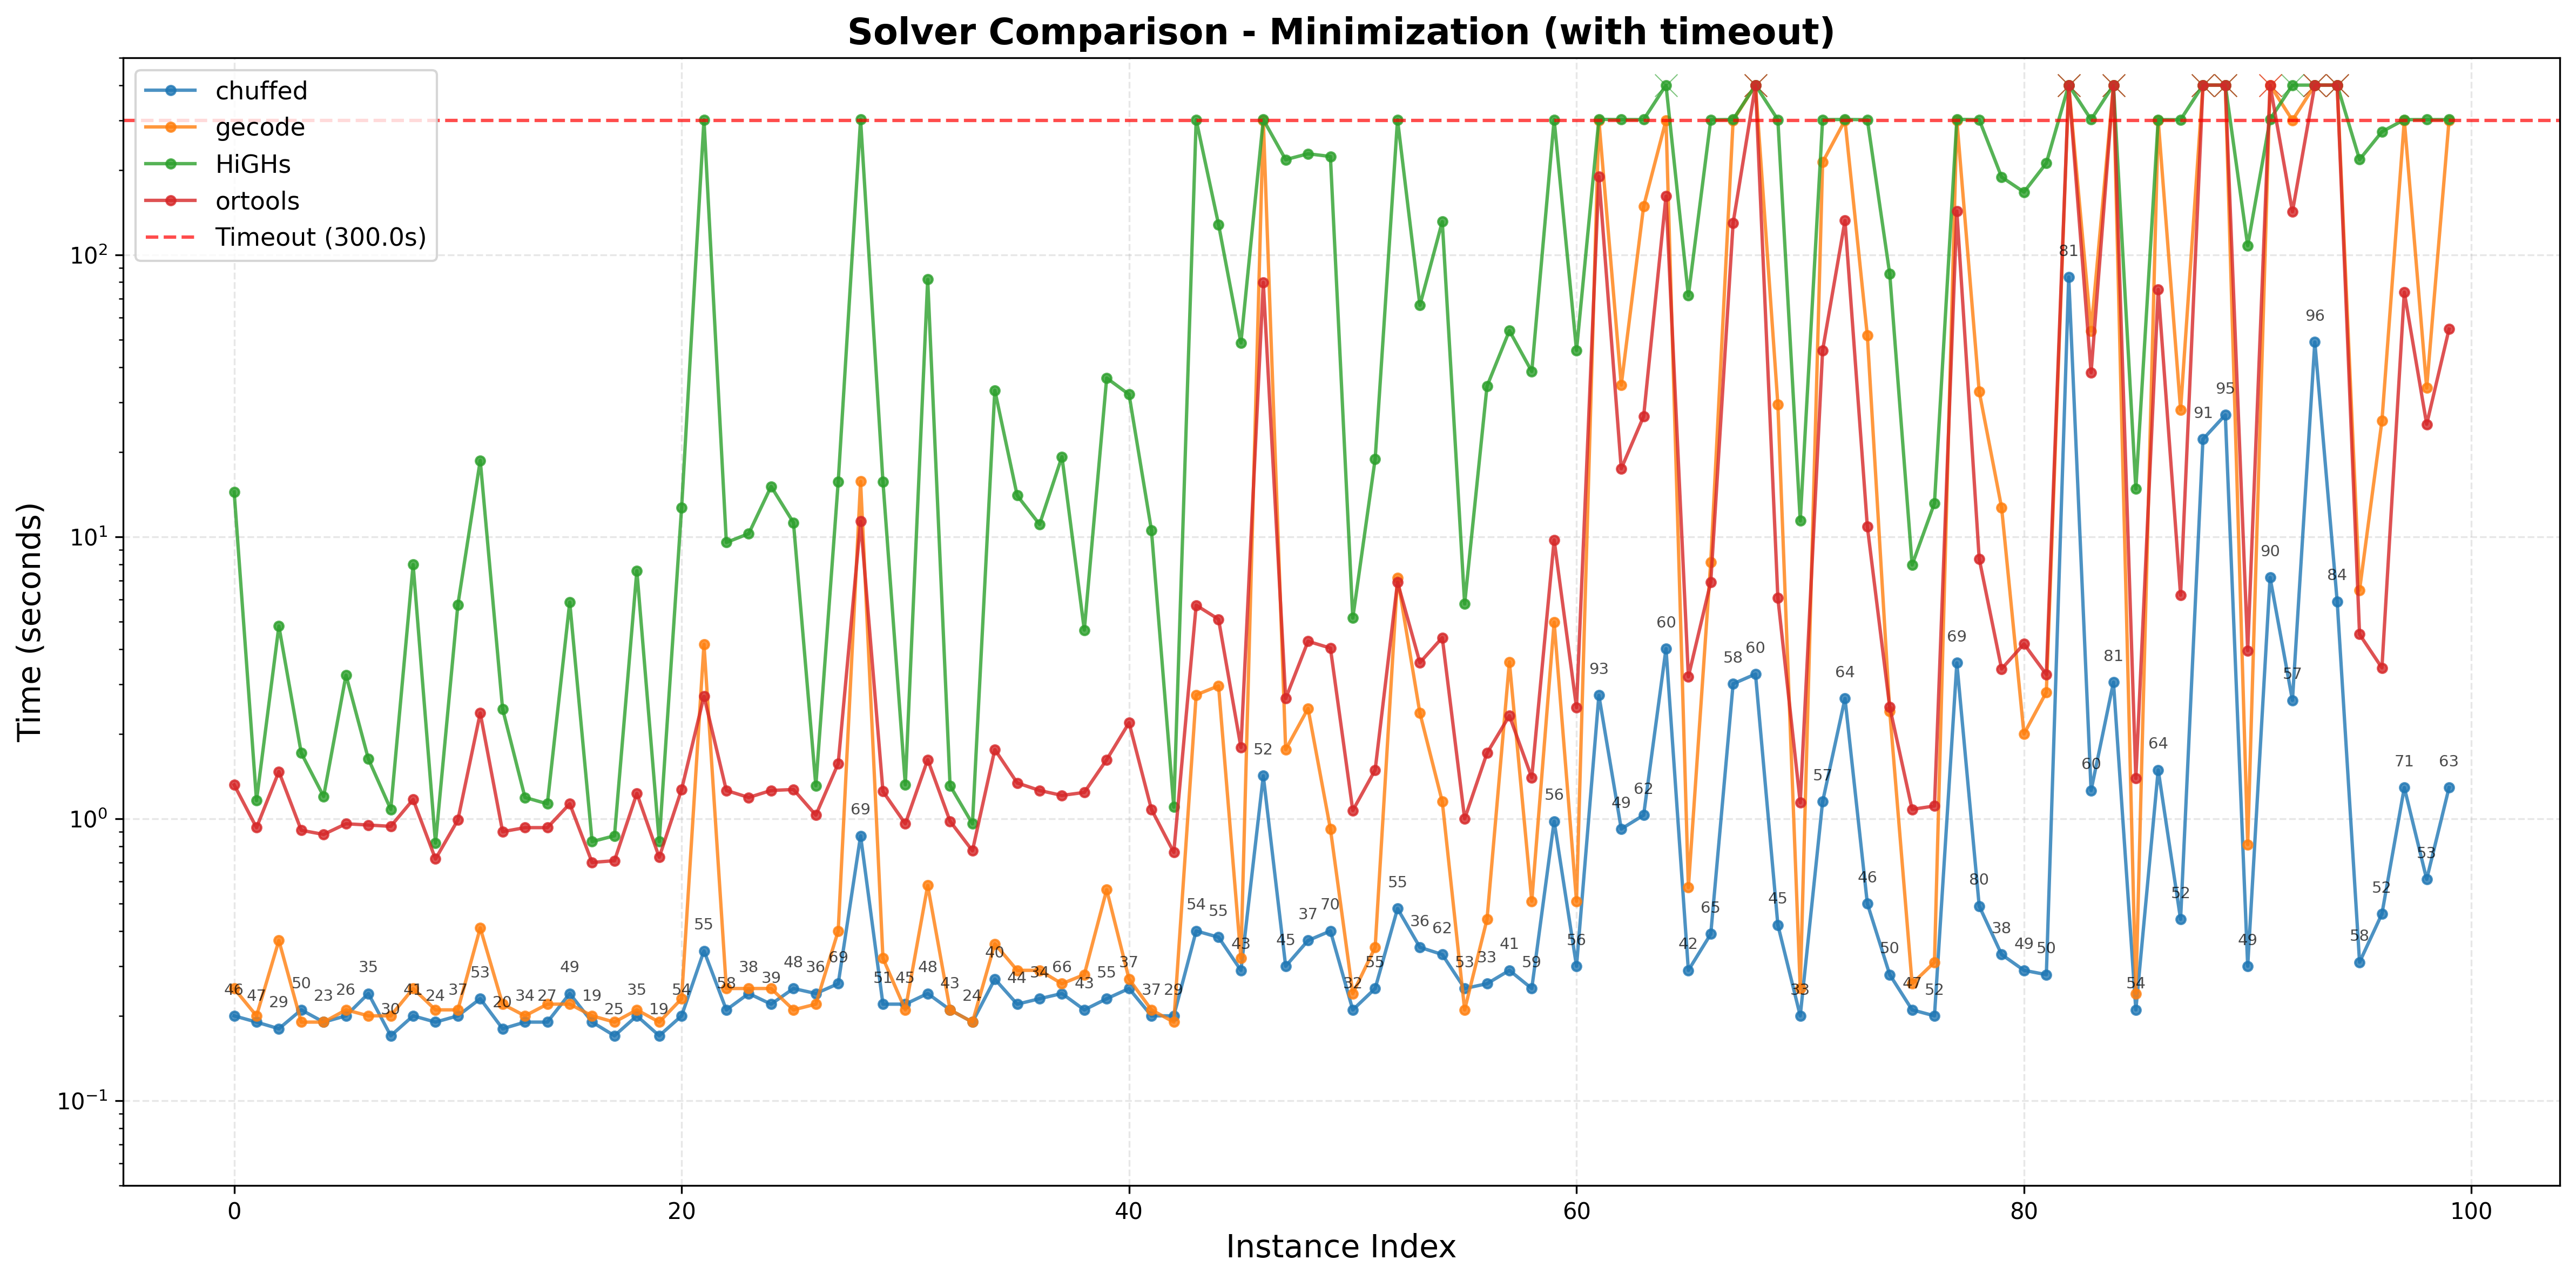
\includegraphics[width=0.85\textwidth]{figures/solver_comparison_minimization_full.png}
    \caption{Solver comparison on minimization problem (including timeouts)}
    \label{fig:min-solver-comparison}
\end{figure}

The plot highlights Chuffed's tight runtime distribution, with all instances solving in under 5 seconds and achieving proven optimality. Gecode encountered 8 memory errors and found 10 potentially suboptimal solutions where optimality could not be proven within the timeout (82\% proven optimal), OR-Tools had 8 memory errors with all SAT\_MIN instances achieving proven optimality (92\% proven optimal), and HiGHs shows 9 memory errors plus 24 potentially suboptimal solutions where optimality could not be proven (67\% proven optimal).

\subsubsection{Search Strategy Evaluation}

Similar to the base problem, we evaluated custom search strategies against Chuffed's default configuration. Figure~\ref{fig:min-strategies} presents the results across all instances, including timeouts.

\begin{figure}[H]
    \centering
    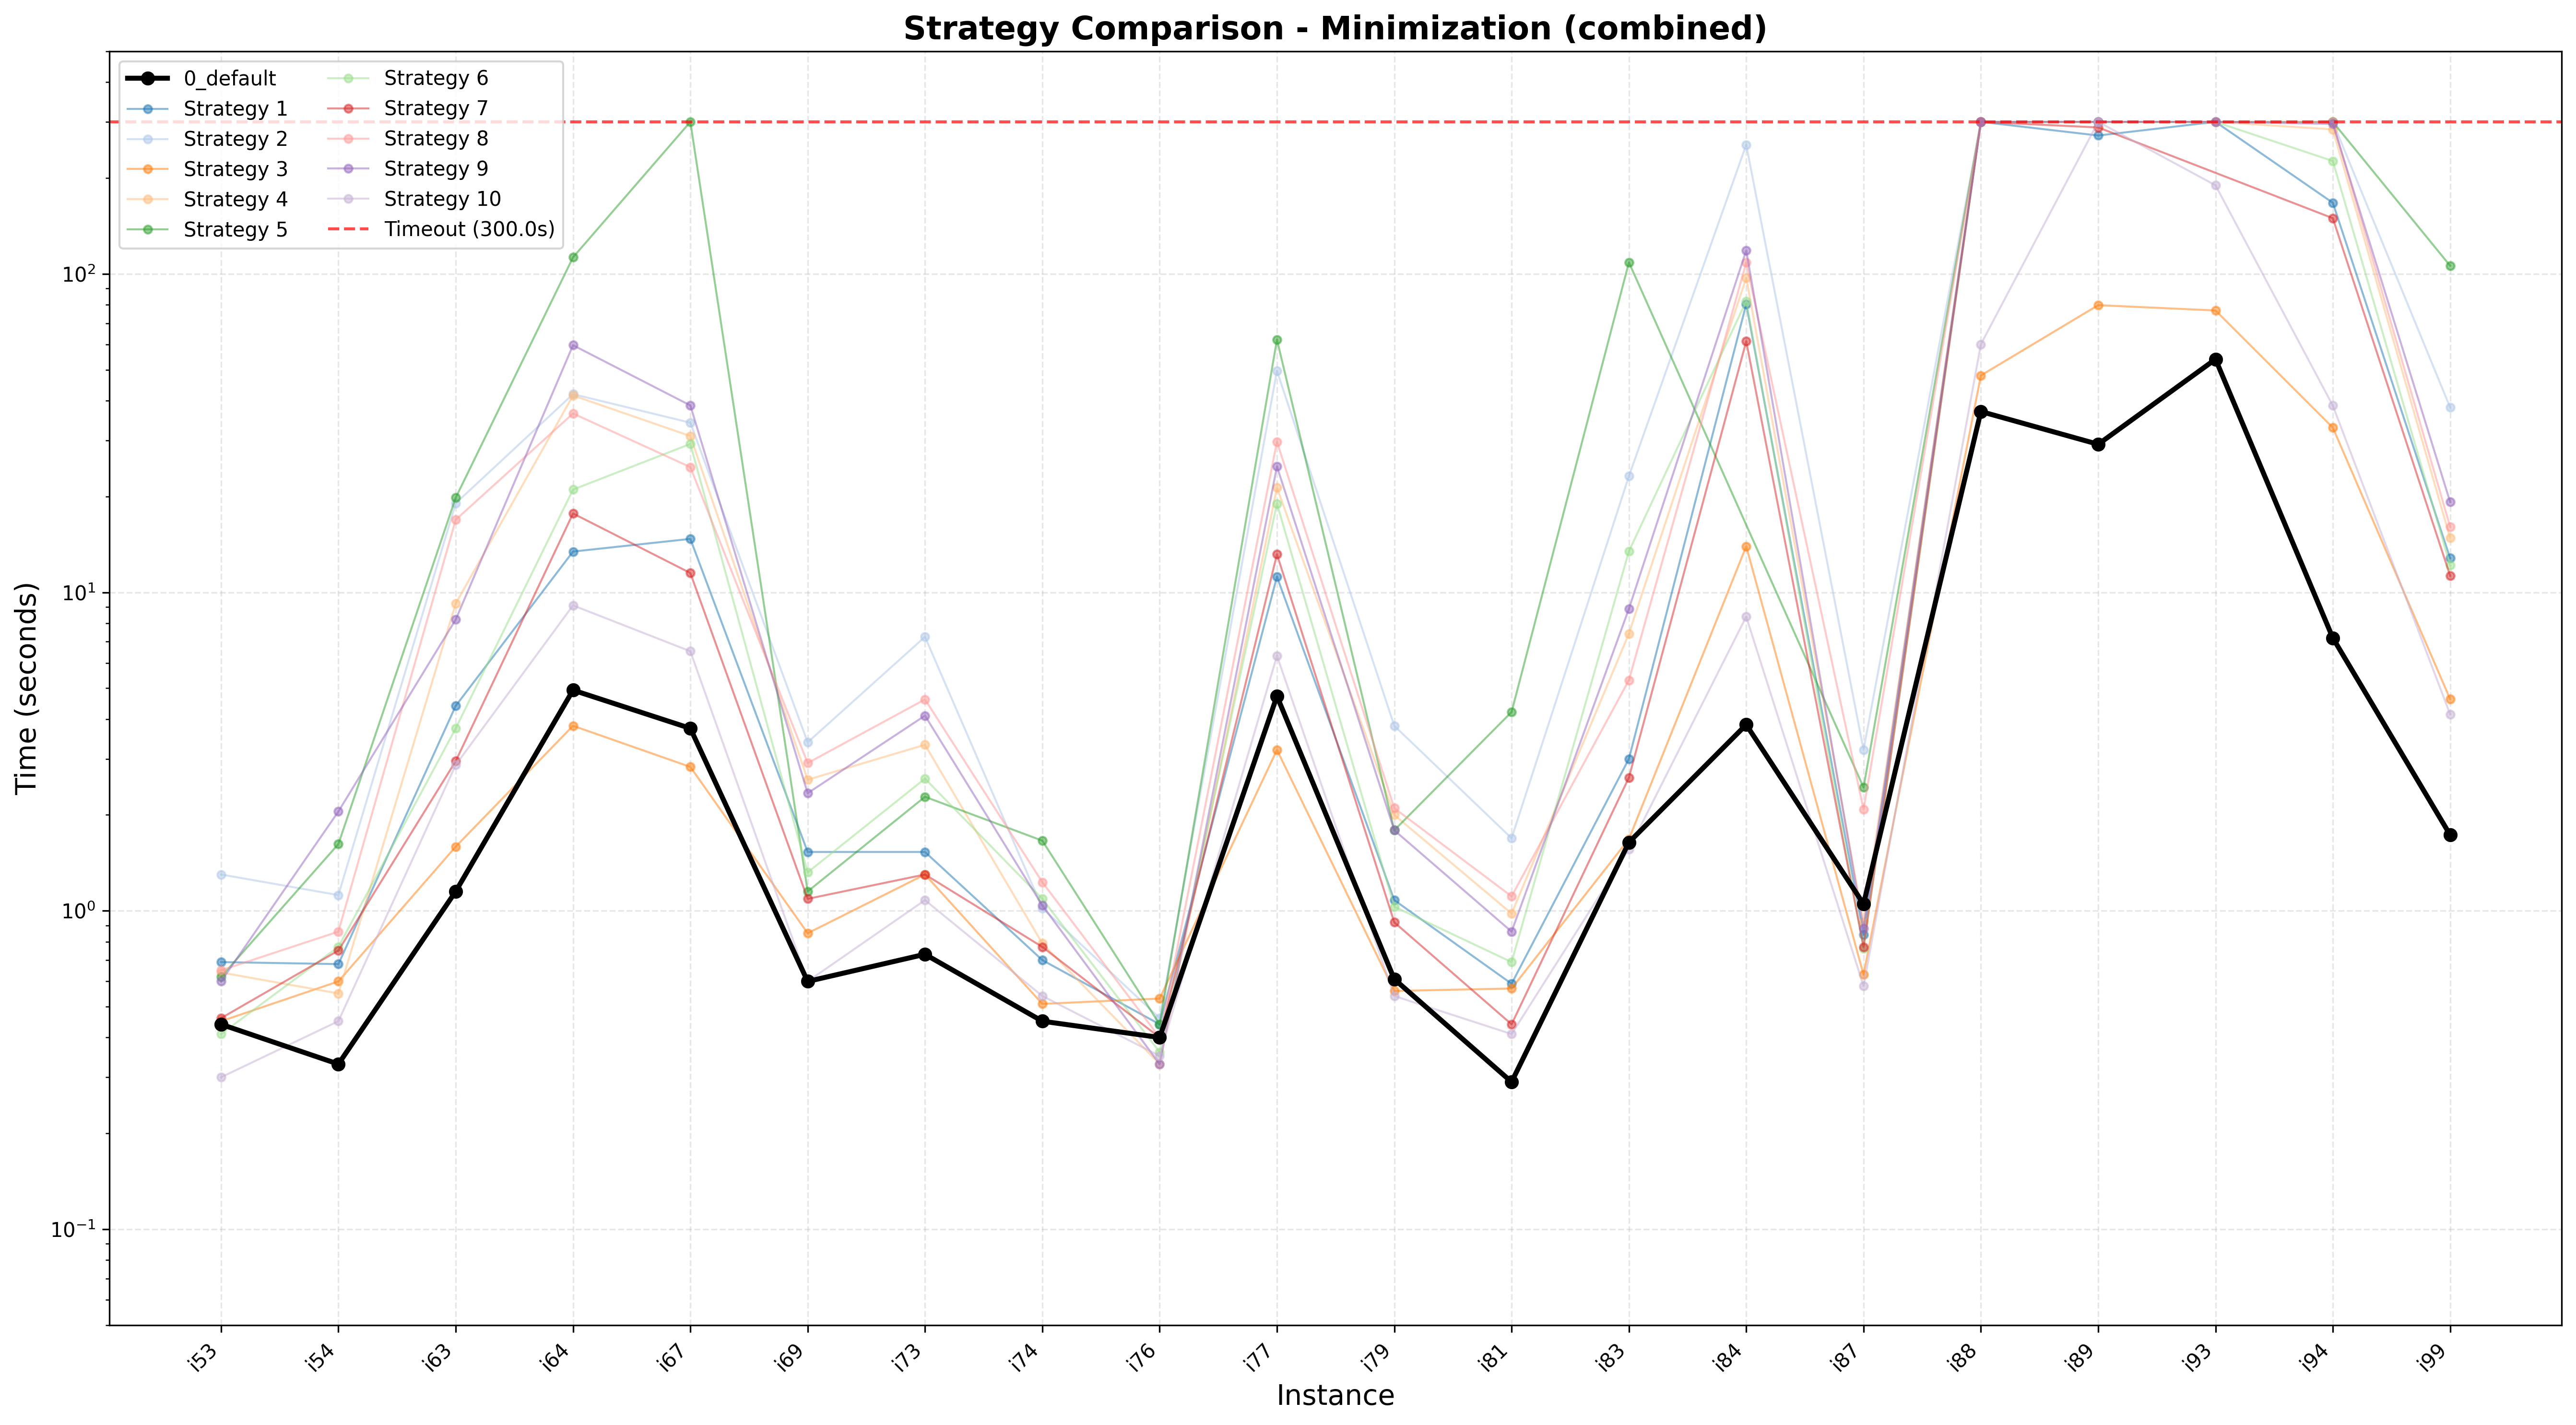
\includegraphics[width=0.85\textwidth]{figures/strategy_combined_minimization_full.png}
    \caption{Search strategies on minimization problem (including timeouts)}
    \label{fig:min-strategies}
\end{figure}

Once again, the default search strategy proves highly effective, with no custom strategy providing a clear, consistent advantage. The optimization objective does not appear to benefit significantly from manual search annotations, further proving the effectiveness of Chuffed's internal heuristics.

\subsubsection{Minimization Phase Performance Summary}

The minimization phase results clearly demonstrate Chuffed's superiority in proving cost optimality. With an average MIN time of 2.52 seconds and a 100\% proven optimality rate, Chuffed significantly outperforms all other solvers. When including failed instances, timeouts and memory errors counted as 300 seconds, Gecode averages 61.54 seconds (82\% proven optimal), HiGHs averages 102.83 seconds (67\% proven optimal), and OR-Tools averages 39.63 seconds (92\% proven optimal).

Even when comparing only instances where optimality was proven, which provides a more favorable view of the competing solvers, Chuffed remains the clear winner: Gecode's 9.17 seconds is 3.6× slower, HiGHs' 45.36 seconds is 18× slower, and OR-Tools' 16.61 seconds is 6.6× slower than Chuffed's 2.52 seconds. This performance advantage, combined with the perfect proven optimality rate and no memory errors, confirms that Chuffed's lazy clause generation mechanism is exceptionally well-suited for optimization problems with complex temporal and resource constraints.

\section{Conclusions}

This project presented a comprehensive constraint programming approach to the Trucks problem, including both satisfiability and optimization variants. The work demonstrates the effectiveness of model design, solver selection, and evaluation while facing logistical planning problems.

\subsection{Key Findings}

\paragraph{Best Configuration} Chuffed with default search settings emerged as the optimal solver configuration for both the base problem and the cost minimization variant. Its lazy clause generation mechanism proved highly effective on the temporal and resource constraints inherent in the Trucks problem, achieving 100\% success rates with consistently low runtimes.

\paragraph{Incremental $K$ Approach} The removal of the \texttt{plan\_length} optimization variable in favor of a pure satisfiability model, combined with an incremental search over $k$ values, proved to be both conceptually simpler and computationally more efficient than embedded optimization. This design decision reduced the search space and eliminated redundant work, as the incremental framework inherently finds minimal-length plans.

\paragraph{Solver Performance Comparison} The experimental results clearly delineate solver capabilities:
\begin{itemize}
    \item \textbf{Chuffed:} 100\% success on BASE (1.85s avg), 100\% optimality on MIN (2.52s avg)
    \item \textbf{OR-Tools:} 100\% success on BASE (3.96s avg), 92\% optimality on MIN (16.61s avg)
    \item \textbf{Gecode:} 86\% success on BASE (13.36s avg), 82\% optimality on MIN (9.17s avg)
    \item \textbf{HiGHs:} 75\% success on BASE (24.93s avg), 67\% optimality on MIN (45.36s avg)
\end{itemize}
Chuffed's superiority is particularly noticeable on harder instances and optimization problems, where lazy clause learning provides a clear advantage over traditional constraint propagation.

\paragraph{Custom Search Strategies} Contrary to initial expectations, custom search strategies, including sequential timestep ordering, position, first heuristics and adaptive domain splitting, did not provide a significant improvements over Chuffed's default configuration. This finding suggests that Chuffed's internal heuristics and learned clauses effectively capture the problem structure, making manual strategy tuning unnecessary for this problem class.

\paragraph{Two-Phase Optimization} The workflow of first finding the minimum plan length via BASE, then optimizing cost at that fixed length, proved efficient and practical. The Base phase quickly identifies the shortest feasible plan, and the MIN phase refines routing decisions without re-exploring infeasible regions of the search space.

\subsection{Model Evolution}

The initial model included redundant optimization variables and overly complex action encoding. Through analysis of solver behavior and benchmark results, the model evolved to:
\begin{itemize}
    \item Eliminate the \texttt{plan\_length} variable in favor of incremental external search
    \item Strengthen propagation through reification and channeling constraints
    \item Leverage precomputed distance matrices for efficient cost computation
\end{itemize}

\subsection{Practical Implications}

For anyone facing similar planning problems, this work offers several insights:
\begin{enumerate}
    \item \textbf{Solver choice matters:} Lazy clause generation solvers (e.g., Chuffed) should be the first choice for scheduling and planning problems with complex temporal dependencies.
    \item \textbf{Default settings are robust:} Invest effort in model design rather than search strategy tuning; modern solvers often perform well out-of-the-box.
    \item \textbf{Incremental approaches work:} For length minimization, external incremental search can be simpler and faster than embedded optimization.
    \item \textbf{Two-phase optimization:} Separating feasibility and cost optimization can improve efficiency when plan length is a critical metric.
\end{enumerate}

\subsection{Future Directions}

Potential extensions of this work include:
\begin{itemize}
    \item Scaling to larger graphs (N $>$ 30) and longer horizons (k $>$ 20) to stress-test solver limits
    \item Testing with alternative cost functions (e.g. energy consumption)
    \item Extending the model to handle heterogeneous objects or multi-capacity trucks
\end{itemize}

In conclusion, this project demonstrates that well designed constraint models paired with appropriate solvers can efficiently solve complex planning problems. The Chuffed solver with default settings represents the best configuration for the Trucks problem, achieving perfect success rates with minimal runtimes across all benchmark instances.

\end{document}